\chapter{The use of medical isotopes in imaging and therapy}\label{Chapter:Medical_Isotopes}
\noindent


\section{History + Where we are today}

\subsection{External and internal radiotherapy }
General about external, internal, how they differ. Write most about internal, and the use of tracers, the different possibilities. 


Today, several treatments are used to cure cancer, among the most commonly used methods; chemotherapy, surgery, external beam therapy and immunotherapy.  External beam therapy utilizes the stopping power of particles like photons (X-rays), electrons, protons and heavier ions, to deposit most of the energy at the site of the tumor. Depending on the tissue, depth and shape of tumor and the energy of the particles, a dose plan can be made which will maximize the effect over the tumor and spare as much as the healthy tissue as possible. However, it has its limitations. Firstly it can only give dose to one single tumor, so the the specific use of external beam is not enough if the cancer has spread. The exposure of healthy tissue will be present, although methods using heavy ions can give a more specific dose, due to the Bragg-peak from Bethe-Block. \newline

\noindent
The idea behind targeted radionuclide therapy is to use radiopharmaceuticals which consist of a radionuclides which emit short-range ionizing particles, and a cell-targeting vector which can target specific cancer cells. Figure \ref{fig:interna_external} shows an illustration of how internal and external therapy differs. Using this type of treatment, it is possible to give a more localized dose, and even treat metastasis. But it does require knowledge of the biology, and how the biological update and half life is. Characteristics which are typical for all radionuclides used in therapy is that it should have sufficient long half life, so that it can be targeted in cancer cells but washed out of the body before too much dose is deposited. For imaging  where you would like to have short half life, so that the patient will not remain radioactive after the imaging. The size of the radiopharmaceutical should not be too large, especially if brain is targeted, because of the blood brain barrier. 

A limitation of targeted radionuclide therapy is that we can not see where the dose is actually deposited. This is why looking for theranostic pairs; one radionuclide which emit gammas or positrons for imaging (PET or SPECT) and one radionuclide used for treatment, emitting short range particles. The pair should have similar physical and chemical properties so they are taken up in equal quanta in the body, the imaging agent should have a short half life and treatment agent should have a longer half life. \textcolor{red}{look up what the actual half lives should be.} 

\begin{figure}
    \centering
    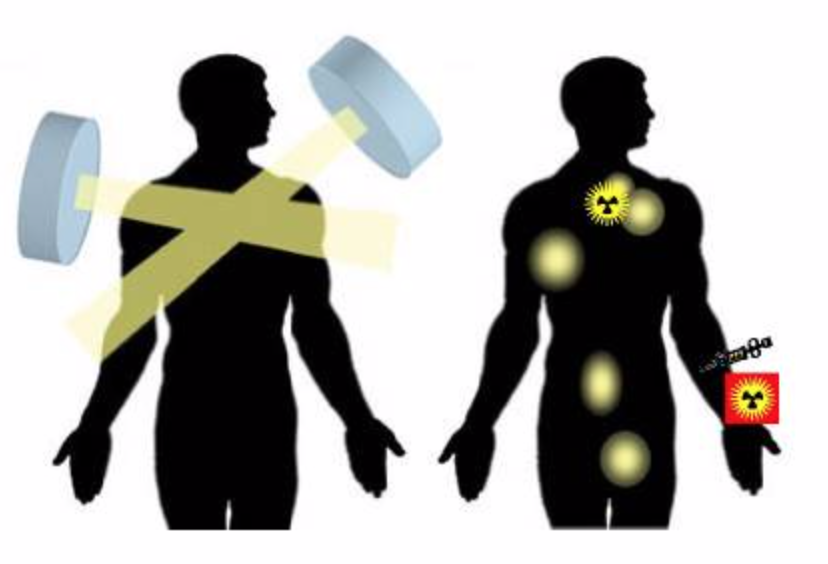
\includegraphics[width=0.5\textwidth]{Theory/internal_vs_external.png}
    \caption{Figure shows how external beam therapy works in comparison to targeted radionuclide therapy. Picture is accessed from \cite{figure_internal_external}}
    \label{fig:interna_external}
\end{figure}


\section{Medical isotopes}

\subsection{General characteristics}
Biological and physical properties. 
LET
Decay types 





\section{Platinum isotopes used in medicine} 

\subsection{Pt-193m}
potential, decay, how it is thought to be used. 

\section{Nuclear production cross sections}
Why we are interested, why is there a need for nuclear production cross sections. 

\subsection{Irradiation on target}
Maybe not?

\subsection{Production and reaction channels}
Compound nucleus, what happens. 
Q value, binding energy, particle emission, probabilities (why does n, p/alpha emission require higher energy, but is more favoured than T emission if both possible.)


\subsection{Expected products from deuterions on iridium, iron, cupper and nc}

Include figure of different nuclear charts, and write about Q values, and reaction channels, which makes it more probable that we observe it (eg. when neutron, proton/alpha channels opens).

